% =============================================================================
% comparacion_figuras_2012.tex — Comparación visual: las figuras de la
% Sección 4 de Gutiérrez et al. (2012) vs. las reproducciones de este
% estudio (scripts/analizar_reprod.py, analizar_reprod_fisica.py, analizar_gr.py).
% Las imágenes originales del capítulo están en figuras_2012_original/,
% extraídas con pdfimages/pdftoppm de ChapterInelastic2012.pdf.
% Compilar: pdflatex comparacion_figuras_2012.tex (dos pasadas)
% =============================================================================
\documentclass[11pt,a4paper]{article}

\usepackage[utf8]{inputenc}
\usepackage[T1]{fontenc}
\usepackage[spanish,es-nodecimaldot]{babel}
\usepackage[margin=2.2cm]{geometry}
\usepackage{amsmath,amssymb}
\usepackage{graphicx}
\usepackage{booktabs}
\usepackage{enumitem}
\usepackage[colorlinks=true,linkcolor=blue!50!black,citecolor=blue!50!black]{hyperref}

\newcommand{\eps}{\varepsilon}
\newcommand{\lammps}{\textsc{Lammps}}

\title{\textbf{Comparación de figuras: Gutiérrez et al. (2012) vs.\ este estudio}\\
\large Reproduciendo las figuras originales para entender el problema}
\author{Felipe Wasaff}
\date{Julio 2026}

\begin{document}
\maketitle

\begin{abstract}
Este estudio nació como una reproducción de la Sección~4 de
Gutiérrez \emph{et al.} (2012)\cite{Gutierrez2012}. Esta nota pone lado a
lado cada figura cuantitativa de esa sección (Figs.~5--9 del capítulo) con
su reproducción en este proyecto (\texttt{in.bounce\_reprod} +
\texttt{scripts/analizar\_reprod*.py}, \texttt{analizar\_gr.py}), discute
dónde coinciden, dónde difieren, y qué nos enseña cada diferencia sobre el
problema físico y sobre las decisiones de implementación de ambos
trabajos.
\end{abstract}

\tableofcontents

% =============================================================================
\section{Introducción}
% =============================================================================

El capítulo original corre una única simulación por altura $h_0$ y
muestra el resultado en cinco figuras: instantáneas de la colisión
(Figs.~5--6), alturas de rebote sucesivas (Fig.~7), la función de
distribución de pares $g(r)$ de la bola en distintos instantes (Fig.~8), y
la evolución temporal de las ocho energías de la
Sección~4.2.3 (Fig.~9). Reproducir estas cinco figuras con nuestro propio
código, y compararlas panel a panel, es la prueba de integración más
directa de que \texttt{in.bounce\_reprod} realmente resuelve el mismo
problema que el capítulo ---antes de extenderlo a los cúmulos de $N$
exacto, el promedio sobre orientaciones y la reformulación de la
equipartición que motivan el resto del proyecto.

% =============================================================================
\section{Instantáneas de la colisión}
% =============================================================================

El capítulo muestra dos secuencias de cuatro instantáneas: Fig.~5
($h_0=11.03\,\sigma$, rebote cuasi-elástico, la bola vibra pero conserva
su forma) y Fig.~6 ($h_0=28.15\,\sigma$, la bola se deforma y adquiere una
forma nueva). Nuestra Fig.~\ref{fig:cmp_snapshots} (nuestra versión de la
derecha) muestra la misma secuencia de cuatro momentos ---caída libre,
compresión máxima, primer rebote, primer apogeo--- para un caso propio.

\begin{center}
\begin{minipage}{0.47\textwidth}
\centering
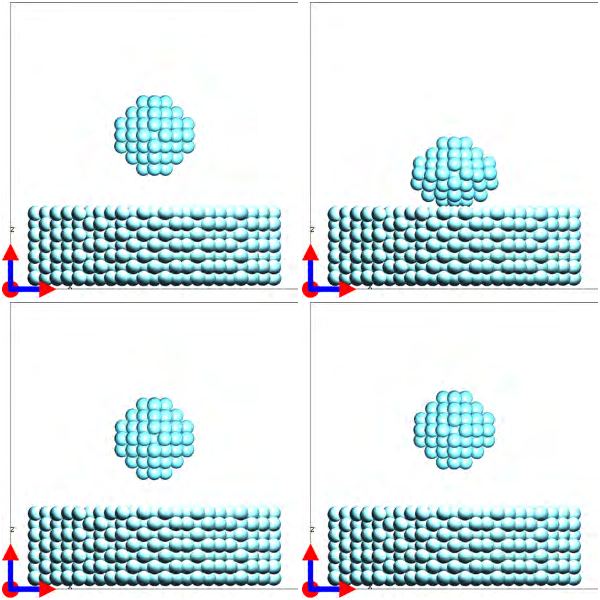
\includegraphics[width=\textwidth]{figuras_2012_original/fig5_montage.png}\\[2pt]
\footnotesize Fig.~5 del capítulo: (a)--(d), $h_0=11.03\,\sigma$.
\end{minipage}
\hfill
\begin{minipage}{0.47\textwidth}
\centering
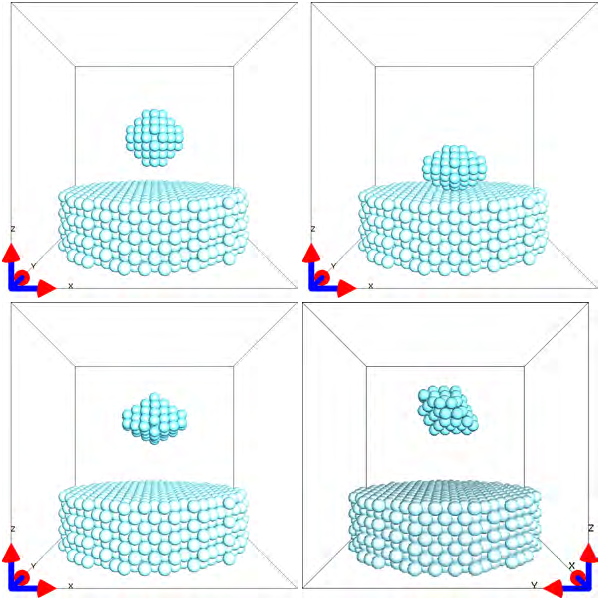
\includegraphics[width=\textwidth]{figuras_2012_original/fig6_montage.png}\\[2pt]
\footnotesize Fig.~6 del capítulo: (a)--(d), $h_0=28.15\,\sigma$.
\end{minipage}
\end{center}

\begin{figure}[h!]
\centering
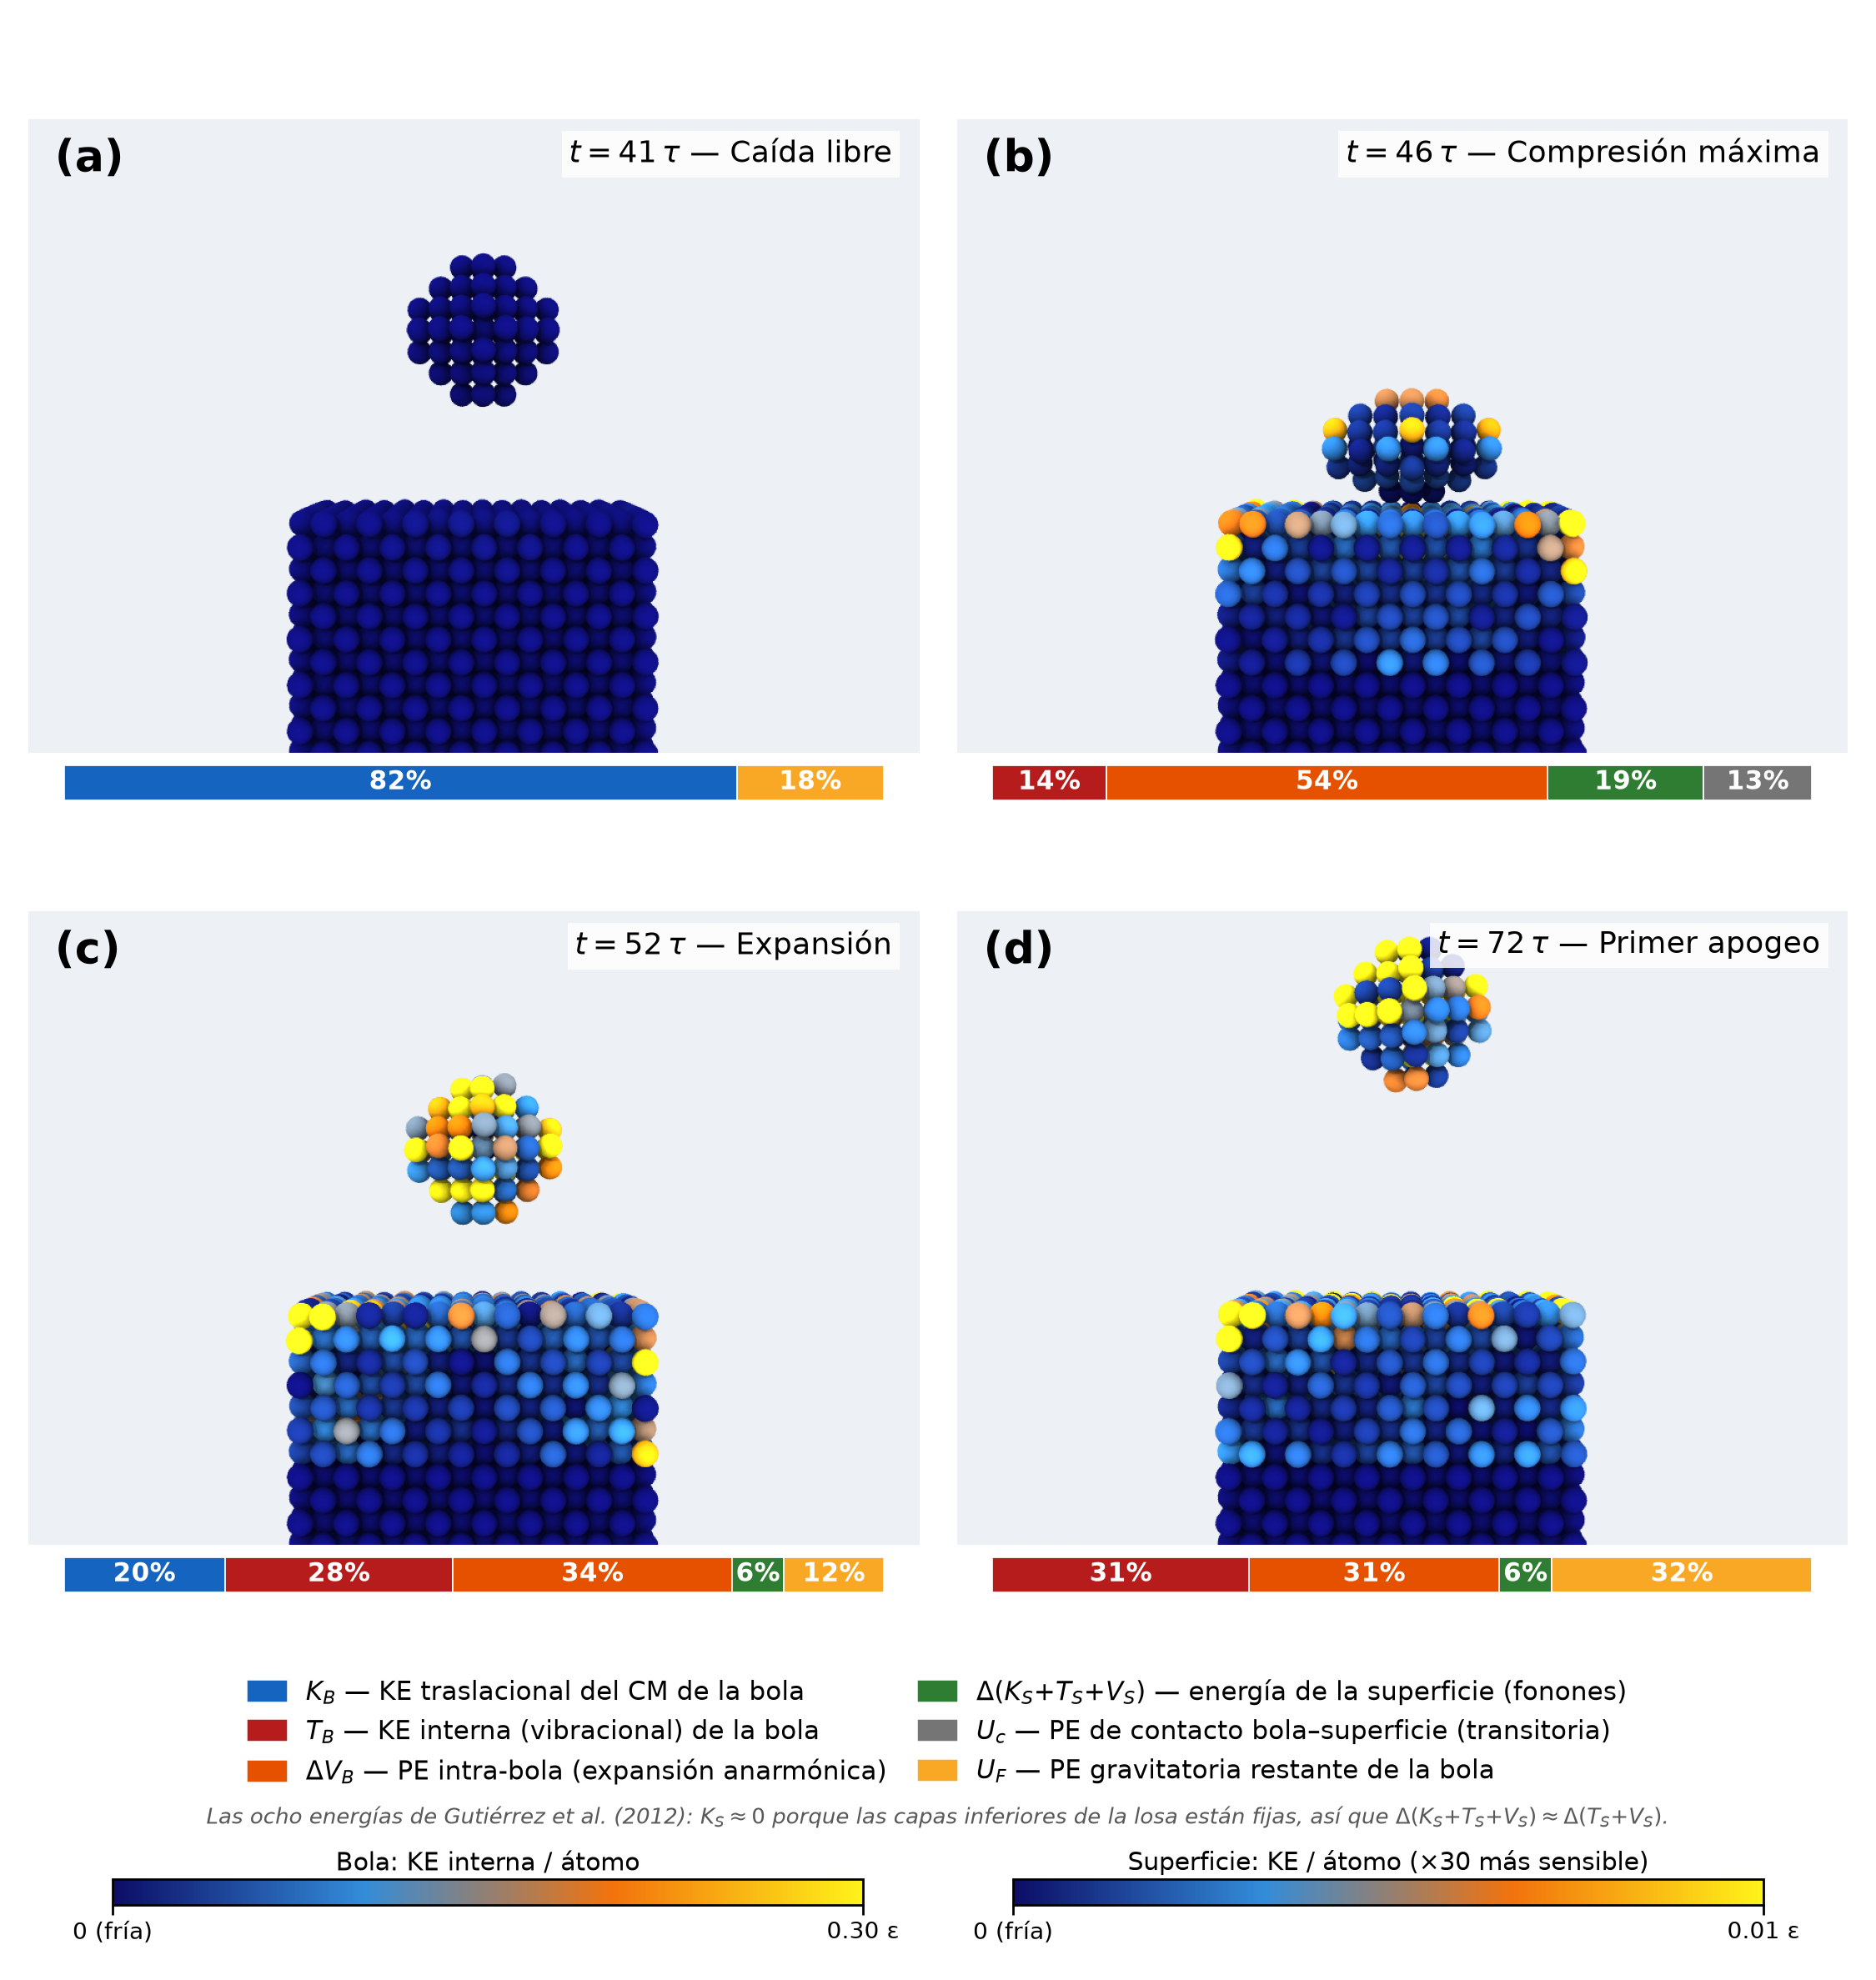
\includegraphics[width=0.92\textwidth]{../figuras_rbef/fig_sequence.png}
\caption{Nuestra secuencia equivalente (\texttt{scripts/analizar\_reprod\_fisica.py},
renderizada con OVITO): caída libre, compresión máxima, primer rebote,
primer apogeo. A diferencia de las Figs.~5--6 del capítulo, cada panel
lleva una barra con la partición de energía en ese instante y un mapa de
color por energía cinética local por átomo (azul fría, amarillo caliente)
--- la misma información cualitativa (geometría) más la cuantitativa
(dónde está la energía) en un solo gráfico.}
\label{fig:cmp_snapshots}
\end{figure}

\textbf{Lo que coincide:} la secuencia física es idéntica --- la bola cae
esférica, se aplana contra la superficie en la compresión máxima, se
recupera parcialmente al separarse y llega al apogeo con una forma
persistentemente irregular (no vuelve a ser una esfera perfecta), señal
directa de la energía que quedó atrapada en modos internos.

\textbf{Lo que se agrega:} el capítulo original solo muestra geometría;
nuestra versión sobreimprime la partición $\alpha_i$ instante a instante y
un mapa de temperatura local, lo que permite \emph{ver} dónde está la
energía además de \emph{leerla} en una tabla ---una extensión
metodológica directa, no una repetición.

% =============================================================================
\section{Alturas de rebote sucesivas}
% =============================================================================

\begin{figure}[h!]
\centering
\begin{minipage}{0.47\textwidth}
\centering
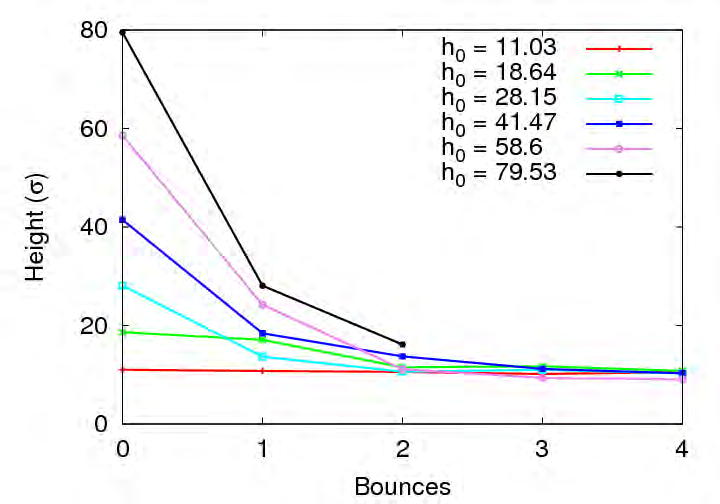
\includegraphics[width=\textwidth]{figuras_2012_original/fig7_final.png}\\[2pt]
\footnotesize Fig.~7 del capítulo (original).
\end{minipage}
\hfill
\begin{minipage}{0.47\textwidth}
\centering
\includegraphics[width=\textwidth]{../../data/outputs/reprod_2012/fig_R1_alturas.pdf}\\[2pt]
\footnotesize Nuestra reproducción (\texttt{analizar\_reprod.py}).
\end{minipage}
\caption{Altura del centro de masa tras cada rebote, para las mismas seis
alturas iniciales $h_0=11.03,\ldots,79.53\,\sigma$.}
\label{fig:cmp_alturas}
\end{figure}

\textbf{Lo que coincide:} la forma cualitativa es la misma en ambas
figuras --- las curvas de $h_0$ alto caen abruptamente en los primeros dos
rebotes y luego convergen todas a una altura de equilibrio baja
($\sim10\,\sigma$), mientras que $h_0=11.03\,\sigma$ (rebote
cuasi-elástico) decae mucho más lento. El capítulo reporta explícitamente
que $h_0=79.53\,\sigma$ solo alcanza a rebotar dos veces antes de perder
su estructura sólida (fusión); nuestra reproducción muestra el mismo
corte temprano para esa curva.

\textbf{Lo que difiere:}
\begin{itemize}[leftmargin=1.4em]
\item \textbf{Rango temporal.} El capítulo solo grafica hasta el cuarto
rebote; nuestra simulación corre lo suficiente para observar hasta 25
rebotes en el caso cuasi-elástico, lo que deja ver el detalle fino de la
convergencia a la altura de equilibrio que la Fig.~7 original no alcanza
a mostrar.
\item \textbf{$N$ no es exactamente 79 en ninguna de las dos
alturas comparadas.} El capítulo fija $M_B=79\,M$ para las ecuaciones de
la Sección~4.2.3, pero nuestra reproducción de \emph{esa misma} receta
(\texttt{create\_atoms region sphere}, radio $2.64\,\sigma$) da
$N=83$ átomos para $h_0=11.03\,\sigma$ y $N=84$ para $h_0=79.53\,\sigma$
(ver \texttt{lammps\_h0\_*.log}) --- un ejemplo concreto y medible del
problema que documentamos en la Sección de métodos de
\texttt{borrador\_rbef\_v2.tex}: recortar una esfera de la red no da un
$N$ fijo, porque el resultado depende de dónde cae el centro de la esfera
respecto de los sitios de la red FCC. Esta es precisamente la razón por
la que el resto del proyecto abandona \texttt{create\_atoms region
sphere} en favor de cúmulos construidos por capas esféricas completas
(\texttt{in.bounce\_cluster}, $N$ exacto).
\end{itemize}

% =============================================================================
\section{Estructura de la bola: la función \texorpdfstring{$g(r)$}{g(r)}}
% =============================================================================

\begin{figure}[h!]
\centering
\begin{minipage}{0.31\textwidth}
\centering
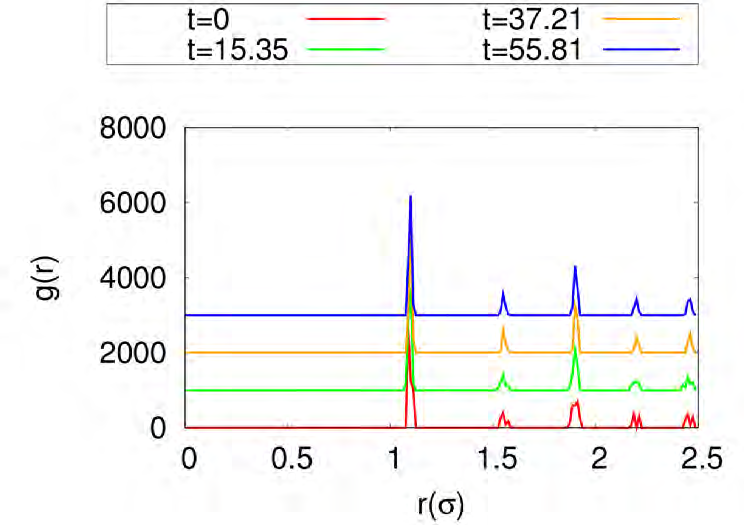
\includegraphics[width=\textwidth]{figuras_2012_original/fig8_final_000.png}\\[2pt]
\footnotesize (a) $h_0=11.03\,\sigma$
\end{minipage}
\hfill
\begin{minipage}{0.31\textwidth}
\centering
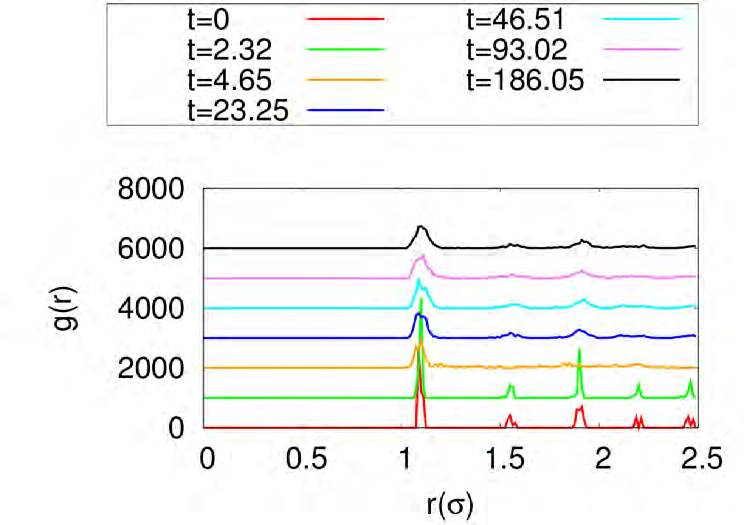
\includegraphics[width=\textwidth]{figuras_2012_original/fig8_final_002.png}\\[2pt]
\footnotesize (c) $h_0=28.15\,\sigma$
\end{minipage}
\hfill
\begin{minipage}{0.31\textwidth}
\centering
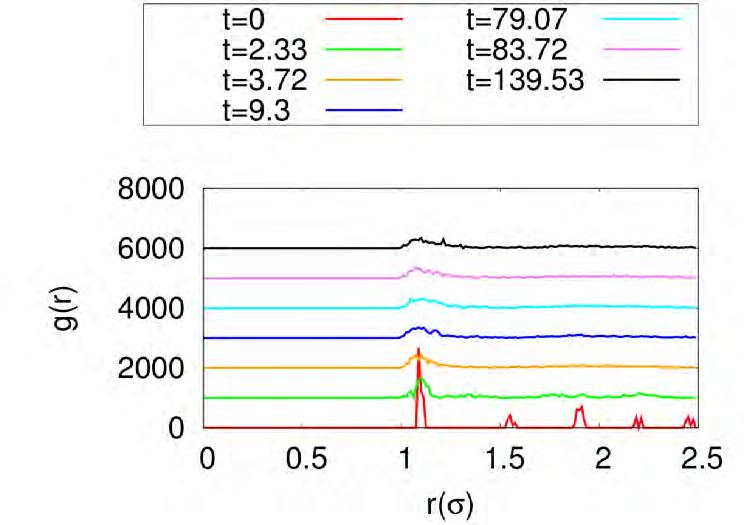
\includegraphics[width=\textwidth]{figuras_2012_original/fig8_final_005.png}\\[2pt]
\footnotesize (f) $h_0=79.53\,\sigma$
\end{minipage}
\caption{Fig.~8 del capítulo (paneles seleccionados): $g(r)$ de la bola en
distintos instantes, para las tres alturas que marcan los tres regímenes
estructurales que discute el capítulo.}
\label{fig:cmp_gr_paper}
\end{figure}

\begin{figure}[h!]
\centering
\includegraphics[width=\textwidth]{../../data/outputs/reprod_2012/fig_gr_ball.pdf}
\caption{Nuestra reproducción (\texttt{analizar\_gr.py}), mismas tres
alturas, mismo panel por panel: FCC conservado, FCC deformado, y FCC
$\to$ amorfo.}
\label{fig:cmp_gr_nuestro}
\end{figure}

\textbf{Lo que coincide:} la conclusión estructural es idéntica en ambos
casos, panel por panel, para las tres alturas:
\begin{itemize}[leftmargin=1.4em]
\item $h_0=11.03\,\sigma$: los picos de segundo y tercer vecino
($r_2=a_0$, $r_3=a_0\sqrt{3/2}$) sobreviven en todos los instantes
posteriores al impacto --- la red FCC se conserva.
\item $h_0=28.15\,\sigma$: los picos de vecinos lejanos se ensanchan y
pierden altura progresivamente --- la red se \emph{deforma} pero no
colapsa del todo.
\item $h_0=79.53\,\sigma$: para $t\gtrsim80\,\tau$ solo sobrevive el
primer pico (a $r_1=a_0/\sqrt2\approx1.09\,\sigma$); todo vecino más allá
del primero se vuelve indistinguible del fondo --- la definición operacional
de \emph{fusión} que usa el capítulo y que adoptamos íntegra en este
proyecto (Sección ``Equipartición: el tamaño de la pelota importa'' de
\texttt{borrador\_rbef\_v2.tex}, y \texttt{scripts/medir\_fusion.py}).
\end{itemize}
Que dos implementaciones de MD completamente independientes (\lammps{}
aquí, \emph{Las Palmeras MD} en el capítulo) lleguen al mismo umbral de
fusión estructural es una validación cruzada fuerte del resultado físico,
independiente de los detalles de cada código.

\textbf{Lo que difiere:} el capítulo reporta los instantes de muestreo
como tiempos absolutos poco redondos ($t=2.32,4.65,23.25,\ldots\,\tau$),
mientras que nuestra reproducción muestrea en los momentos
\emph{dinámicamente relevantes} de cada corrida (impacto, compresión
máxima, primer y segundo apogeo) identificados automáticamente a partir de
los mínimos y máximos de $Z_{\rm CM}(t)$, no fijados a mano. El resultado
es el mismo, pero nuestro criterio de muestreo se generaliza sin
intervención manual a cualquier $N$ o $h_0$ nuevos, lo cual fue necesario
para poder correr el sweep completo de 210 simulaciones.

% =============================================================================
\section{Evolución temporal de las energías}
% =============================================================================

\begin{figure}[h!]
\centering
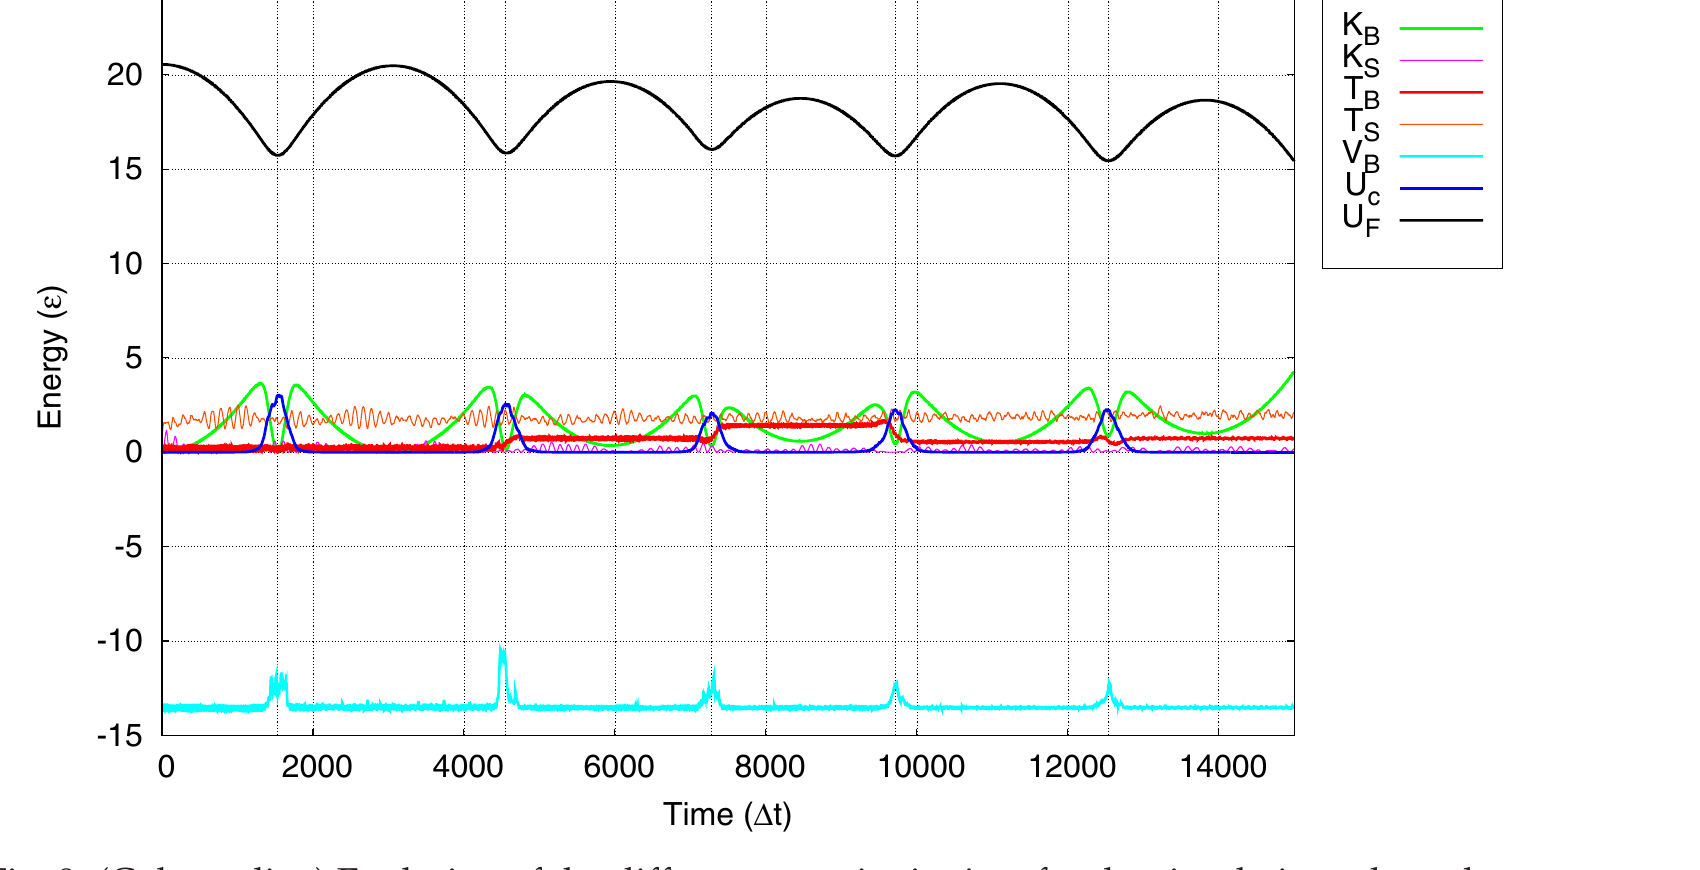
\includegraphics[width=\textwidth]{figuras_2012_original/fig9_final.png}
\caption{Fig.~9 del capítulo (original): evolución de $K_B,K_S,T_B,T_S,
V_B,U_c,U_F$ para $h_0=11.03\,\sigma$, eje temporal en pasos de
integración $\Delta t$ (no en $\tau$).}
\label{fig:cmp_e9_paper}
\end{figure}

\begin{figure}[h!]
\centering
\includegraphics[width=\textwidth]{../../data/outputs/reprod_2012/fig_R2_energia_h0_11.03.pdf}
\caption{Nuestra reproducción (\texttt{analizar\_reprod\_fisica.py}),
mismo caso $h_0=11.03\,\sigma$, eje temporal ya convertido a $\tau$
físicos ($\Delta t_{\rm nuestro}=0.005\,\tau$ por paso).}
\label{fig:cmp_e9_nuestro}
\end{figure}

\textbf{Lo que coincide, cualitativamente:} la forma de cada curva es la
misma familia de curvas en ambas figuras:
\begin{itemize}[leftmargin=1.4em]
\item $K_B$ (verde/negro): una serie de picos con máximo decreciente,
cada uno flanqueado por dos mínimos donde $K_B=0$ (la bola detenida sobre
la superficie) --- exactamente la lectura que hace el propio capítulo de
su Fig.~9 (``estos mínimos representan el instante en que la energía
cinética traslacional $K_B$ se anula'').
\item $U_c$ (azul): picos angostos y altos, sincronizados exactamente con
cada mínimo de $K_B$ --- la energía colisional solo existe mientras hay
contacto.
\item $T_B$ y $V_B$ (rojo): ambas acumulan un piso creciente de ruido
entre bounce y bounce, la firma visual directa de la equipartición y el
virial discutidos en \texttt{equiparticion\_y\_virial.tex}.
\item El capítulo señala explícitamente que, entre el segundo y el
tercer rebote, la energía térmica acumulada $T_B$ se transfiere de vuelta
a $K_B$ y la bola alcanza una velocidad de despegue \emph{mayor} que en el
rebote anterior. Nuestra reproducción muestra el mismo efecto (el pico de
$K_B$ del cuarto rebote es mayor que el del tercero) --- el mismo
intercambio no monotónico entre canales, reproducido de forma
independiente.
\end{itemize}

\textbf{Lo que difiere:}
\begin{itemize}[leftmargin=1.4em]
\item \textbf{Eje temporal.} El capítulo grafica en pasos de integración
$\Delta t$ crudos (hasta 15000); nuestra Fig.~\ref{fig:cmp_e9_nuestro} ya
convierte a $\tau$ físico, así que las escalas horizontales no son
comparables directamente número contra número, solo en forma.
\item \textbf{Offsets manuales.} El capítulo desplaza $U_F$ en $-2\,\eps$
y $V_B$ en $+400\,\eps$ ``para mantener todas las energías en el mismo
rango'' (su nota de la Fig.~9); nuestra versión separa $U_F$ en un panel
inferior aparte en vez de desplazarlo, y omite $V_B$ (cuyo offset de
cohesión, del orden de cientos de $\eps$, no aporta información sobre el
calentamiento --- ver la discusión de $\alpha_{\Delta V_B}$ en
\texttt{comparacion\_energias\_2012.tex}) mostrando en cambio
directamente $\Delta V_B=V_B-V_B^{(0)}$.
\item \textbf{$T_S$ y $K_S$.} El capítulo los grafica explícitamente
(curvas planas cerca de cero, sin aportar información nueva, según su
propio texto); nuestra versión no las incluye en esta figura puntual, pero
sí las agregamos como el canal $\alpha_{\rm surf}$ de pleno derecho en el
resto del proyecto, precisamente porque a velocidades de impacto más
altas que las de este panel dejan de ser insignificantes (Sección
``Un canal de superficie explícito'' de \texttt{comparacion\_energias\_2012.tex}).
\end{itemize}

% =============================================================================
\section{Qué aprendemos de la comparación}
% =============================================================================

Las cuatro comparaciones anteriores dejan tres lecciones concretas:

\begin{enumerate}[leftmargin=1.4em]

\item \textbf{La física coincide, panel por panel.} Cada fenómeno que el
capítulo describe cualitativamente ---rebote cuasi-elástico a baja
energía, deformación permanente a energía intermedia, fusión estructural
a energía alta, intercambio no monotónico entre $K_B$ y $T_B$ entre
rebotes sucesivos--- aparece de forma independiente en nuestra
reproducción, con un código de MD distinto (\lammps{} vs.\ \emph{Las
Palmeras MD}). Esta coincidencia cruzada es la validación más fuerte
posible de que ambas simulaciones resuelven el mismo problema físico.

\item \textbf{El problema de $N$ no es anecdótico.} La comparación de la
Fig.~\ref{fig:cmp_alturas} lo hace medible: reproducir la receta exacta
del capítulo (\texttt{create\_atoms region sphere}) da $N=83$ y $N=84$
para dos alturas que, según la Sección~4.2.3 del propio capítulo, deberían
compartir $N=79$. Esta discrepancia de unas pocas unidades en $N$ --- que
a primera vista parece un detalle menor de implementación --- es
exactamente la motivación que llevó al resto de este proyecto a abandonar
el corte esférico en favor de cúmulos FCC de capas completas.

\item \textbf{Reproducir primero, extender después.} Ninguna de las
figuras nuevas de este proyecto (el canal $\alpha_{\rm surf}$, el barrido
en $N$, el promedio sobre orientaciones, la reformulación
$f_{\rm ball}=(3N-3)/(3N-3+3N_c^{\rm ef})$) tendría sentido sin primero
confirmar, figura por figura, que la reproducción de la Sección~4 original
es sólida. Esta nota documenta esa confirmación.

\end{enumerate}

% =============================================================================
\begin{thebibliography}{9}
\bibitem{Gutierrez2012}
G. Gutiérrez, S. Davis, C. Loyola, J. Peralta, F. González, Y. Navarrete
y F. González-Wasaff, \textit{Inelastic Collisions and Hypervelocity
Impacts at Nanoscopic Level: A Molecular Dynamics Study}, cap.~12 en
\textit{Molecular Dynamics -- Theoretical Developments and Applications
in Nanotechnology and Energy}, editado por L. Wang (InTech, Rijeka, 2012).
\end{thebibliography}

\end{document}
